\documentclass[../Psychological_system_web_application.tex]{subfiles}


\graphicspath{ {images/} }
\begin{document}

	\section{Product perspective}
			\paragraph{The product is supposed to be an open source, under the GNU general Public License. It is a web based system implementing client-server model. The \acr{SRS} For Inelegant psychological System provides simple mechanism for users to share and acquire knowledge.}
			\paragraph{This product have \acr{DB} that store}
				\subsection{ Database System:} 
					\begin{itemize}
						\item
							\textbf{\textsc{\color{red}Session details:}}\\
							Will record the information of any session  like duration of the session , date , the client that take this session, the psychologist that supervise in this session , and report of this session.
						\item
							\textbf{\textsc{\color{red}Client description:}}\\
							It includes client code, name address, email, phone number and birth-date and maybe other information, this information used for confirmed reservation of session and keeping the records of the client for any emergency or any other kind of information.
						\item
							\textbf{\textsc{\color{red}Specialist description:}}\\
							It includes specialist code, name, address, and email, phone number, \acr{SSN} , his qualifications, and graduation year, this information to performance evaluation and develop him.
						\item
							\textbf{\textsc{\color{red}Reservation description:}}\\	
							It includes the day of reservation, date, time, client details, and specialist details, this information to save right of client and specialist in the center.
						\item
							\textbf{\textsc{\color{red}Pay description:}}\\
							It includes pay code, receptionist name, date, time, and price of session, thin total.
						\item
							\textbf{\textsc{\color{red}Income description:}}\\
							It includes the client details, specialist details, session details, number of hour, and notes, this information to compute the total income per day, then per month, then per year and output the report.
						\item
							\textbf{\textsc{\color{red}exported description:}}\\
							It includes The specialist details, total number of sessions, date, day, and total Proportion of Specialist, and total number of hours, this information to compute the total exported at month, and year.  
						\item
							\textbf{\textsc{\color{red}report description:}}\\
							It includes the head title, body of report, and footer and signature 
					\end{itemize}
				\subsection{client side:}
					\paragraph{The system deviated two subsystems, the first subsystem is client side services, and the second server side services, we will introduce in this subsection the client side services.}
					\paragraph{We provide in the client side services the main services like the user will able to log-in into system and log-out from it, he can send request of reservation to specific appointment, and retrieve his schedule, he can access his report that specified to his case, the user can update his profile and change his information, the specialist can enter the available appointment that appropriate to him, and retrieve his schedule, upload case's reports, and can connect with his cases and receptionist or management.}
					\paragraph{The client side services provide to management some reports for calculations of the center, report for total hours of all specialists, and total work hours of center, report for Exports of the center like total salaries of all Employees in the center, Total cost of all maintenance of all things monthly or yearly, report to help decision makers for take the correct decision, report for all problems in the center, and provide for all managers to connect with Employees and clients of center, the client side provide to center mechanism to confirm automatically or manually reservations of the next day.}
					
				\subsection{Server side:}
					\paragraph{We provide in the server side services the main services like Encrypt all data to provide security to system, controller functions that access and connect with \acr{DBMS} that is a collection of programs that enables users to create and maintain a database, and provide the functions that can access or send and receive the requests from client side services}
%%%%%%%%%%%%%%%%%%%%%%%%%%%%%%%%%%%%%%%%%%%%%%%%%%%%%%%%%%%%%%%%%%%%%%%%%%%%%%%%%%%%%%%%%%%%%%%%%%%%%%%%%%%%%%%%%%%%%%%%%%%%%%%%%%%%%%%%%%%%%%%%%%%%%%%%%%%%%%%%%%%%%%%%%%%%%%%%%%%%%%%%%%%%%%%%%%%%%%%%%%%%%%%%%%%%%%
		\section{PRODUCT FEATURES}
			
			\paragraph{  The major features of Inelegant psychological \gls{database} system as shown in below \gls{entity relationship model}}
				
		
%%%%%%%%%%%%%%%%%%%%%%%%%%%%%%%%%%%%%%%%%%%%%%%%%%%%%%%%%%%%%%%%%%%%%%%%%%%%%%%%%%%%%%%%%%%%%%%%%%%%%%%%%%%%%%%%%%%%%%%%%%%%%%%%%%%%%%%%%%%%%%%%%%%%%%%%%%%%%%%%%%%%%%%%%%%%%%%%%%%%%%%%%%%%%%%%%%%%%%%%%%%%%%%%%%%%%%
		\section{User characteristics}
			\subsection{Receptionist}			
			\paragraph{Receptionist should be able to determining the specific appointment for the client, and update any appointment according to client, he should able to retrieve all information of any reservation appointment, retrieve any information of calculation system to specific client, and he retrieve all his conversations with the client in the system}
			
			\subsection{Specialist}
			\paragraph{Specialist should be able to enter his appointments of his sessions daily, or monthly, and he retrieve his schedule of day, he can update his appointments before passing 24 hours from setting it,should be able to retrieve all information of his cases and specific reports that it was written by him, and able to upload the report of specific case.}
			
			\subsection{Client}
			\paragraph{Client should able to retrieve his schedule of his appointments, able to choose from available appointments that his specialist determined its, and able to retrieve all reports that specific his case and download this report, able to update his information and update the appointment before passing 24 hours from his choosing it, he can see the program that his specialist preparing it to him and Proposed Plans to solve issues of the case, he can connect with management of center.}
			
			\subsection{Trainee}
			\paragraph{Trainee should able to choose from available courses and Enroll it, able to retrieve his schedule of appointments of all courses that he Enroll its and all information about its, able to access all materials that specified to the course and download its, able to retrieve specific report about Trainer, his Performance, his Tests, and results or points that take from Exercises}
			
			\subsection{Trainer}
			\paragraph{Trainer should be able to set all courses that will Lecture its, and determine the appropriate appointments for him, supervise trainee that enrolled to courses that will be specified, he can upload the materials of the course and retrieve all information that specific of the trainee in the course, and dropped out The rioters from the course, connect with trainees and receptionist}
		
%%%%%%%%%%%%%%%%%%%%%%%%%%%%%%%%%%%%%%%%%%%%%%%%%%%%%%%%%%%%%%%%%%%%%%%%%%%%%%%%%%%%%%%%%%%%%%%%%%%%%%%%%%%%%%%%%%%%%%%%%%%%%%%%%%%%%%%%%%%%%%%%%%%%%%%%%%%%%%%%%%%%%%%%%%%%%%%%%%%%%%%%%%%%%%%%%%%%%%%%%%%%%%%%%%%%%%
		\section{OPERATING ENVIRONMENT}
			\paragraph{Operating environment for Inelegant psychological System is as listed below.}
				\begin{itemize}
					\item
							\textbf{distributed \gls{database}}
					\item
							\textbf{client/server system}
					\item
							\textbf{Operating system: Windows, windows phone, android, mac os, linux}
					\item
							\textbf{database: my sql database}
					\item
							\textbf{platform: Python/Java/\acr{JSP}}
				\end{itemize}
		
%%%%%%%%%%%%%%%%%%%%%%%%%%%%%%%%%%%%%%%%%%%%%%%%%%%%%%%%%%%%%%%%%%%%%%%%%%%%%%%%%%%%%%%%%%%%%%%%%%%%%%%%%%%%%%%%%%%%%%%%%%%%%%%%%%%%%%%%%%%%%%%%%%%%%%%%%%%%%%%%%%%%%%%%%%%%%%%%%%%%%%%%%%%%%%%%%%%%%%%%%%%%%%%%%%%%%%
		\section{DESIGN AND IMPLEMENTATION CONSTRAINTS}
			
			\subsection{Schema}
			
				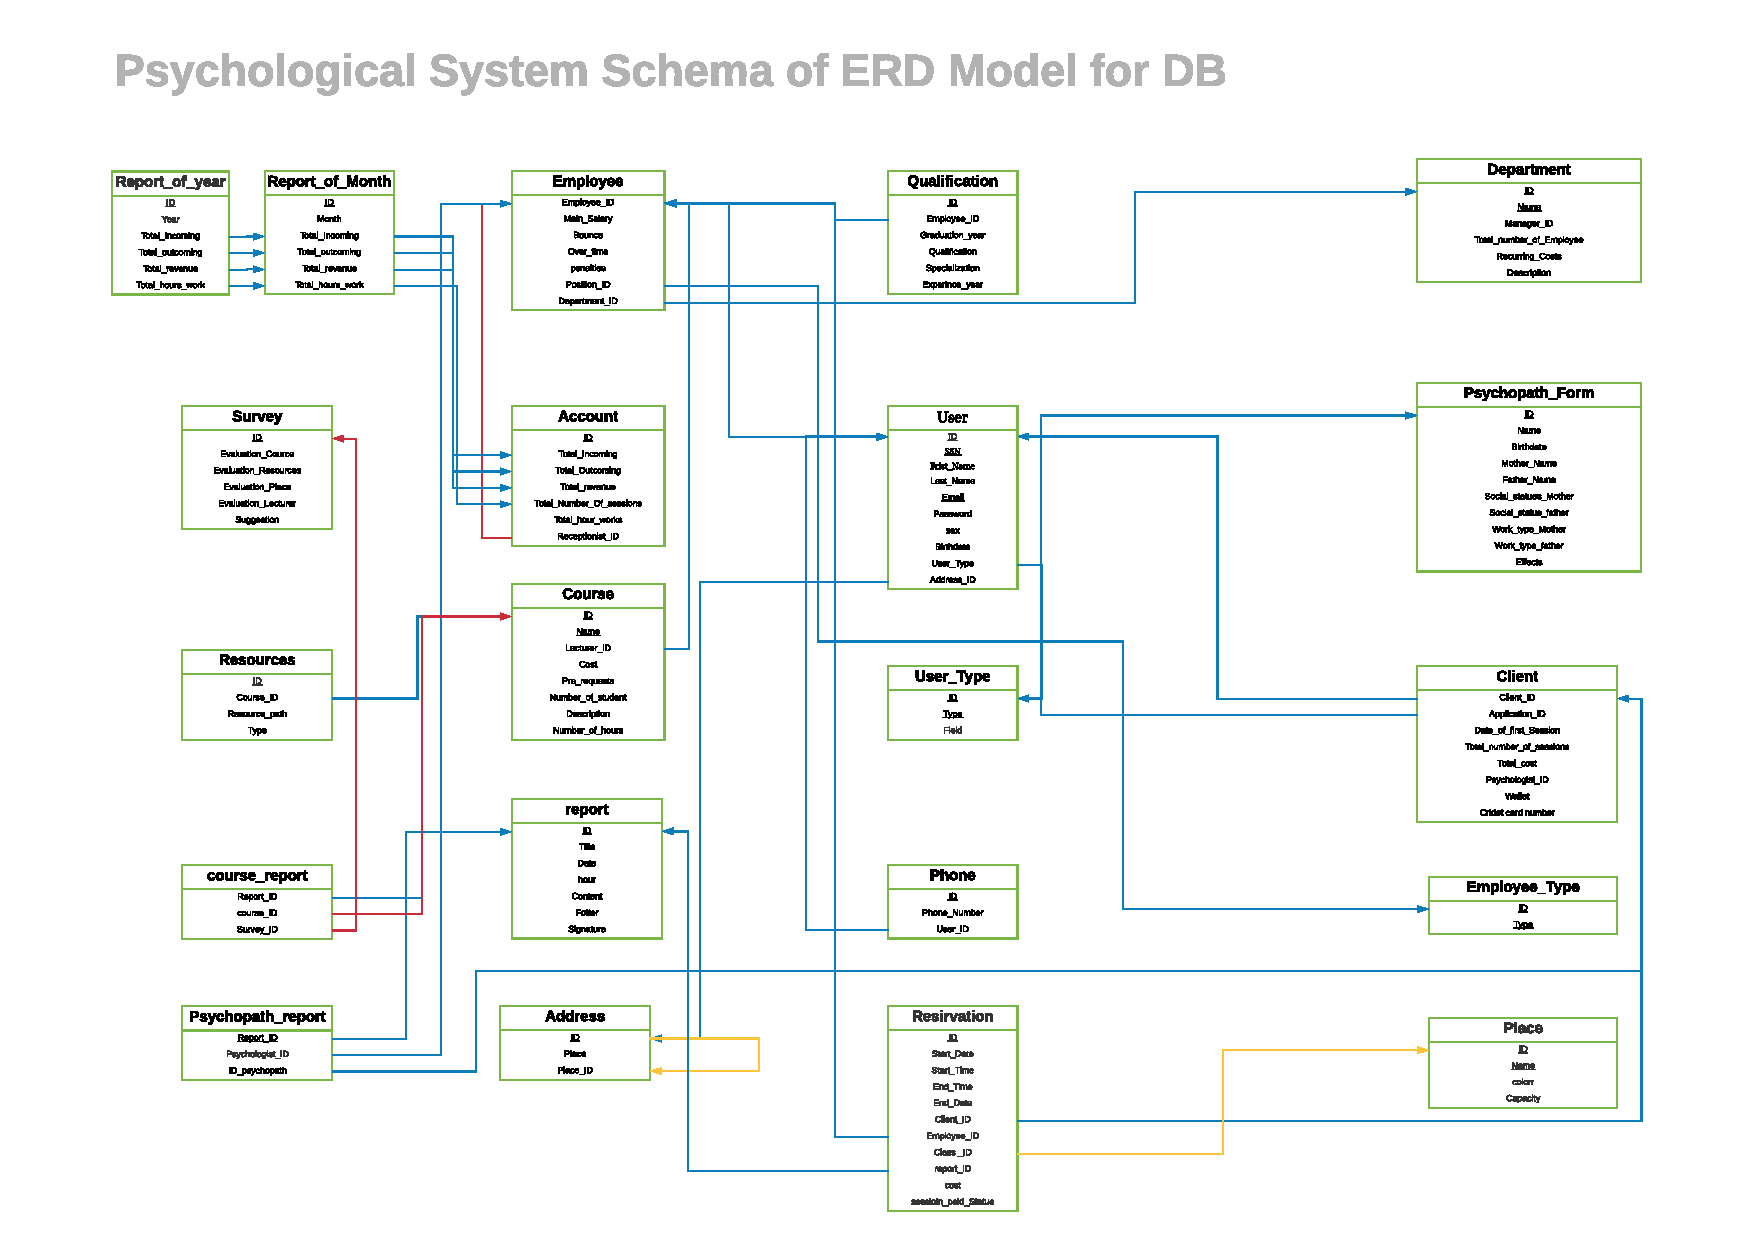
\includegraphics[width=\textwidth ,height=0.9\textheight ,scale=4]{Diagrams/Psychological_schema.pdf}				
				
			\subsection{Data flow diagram}
				\subsubsection{Context diagram}
					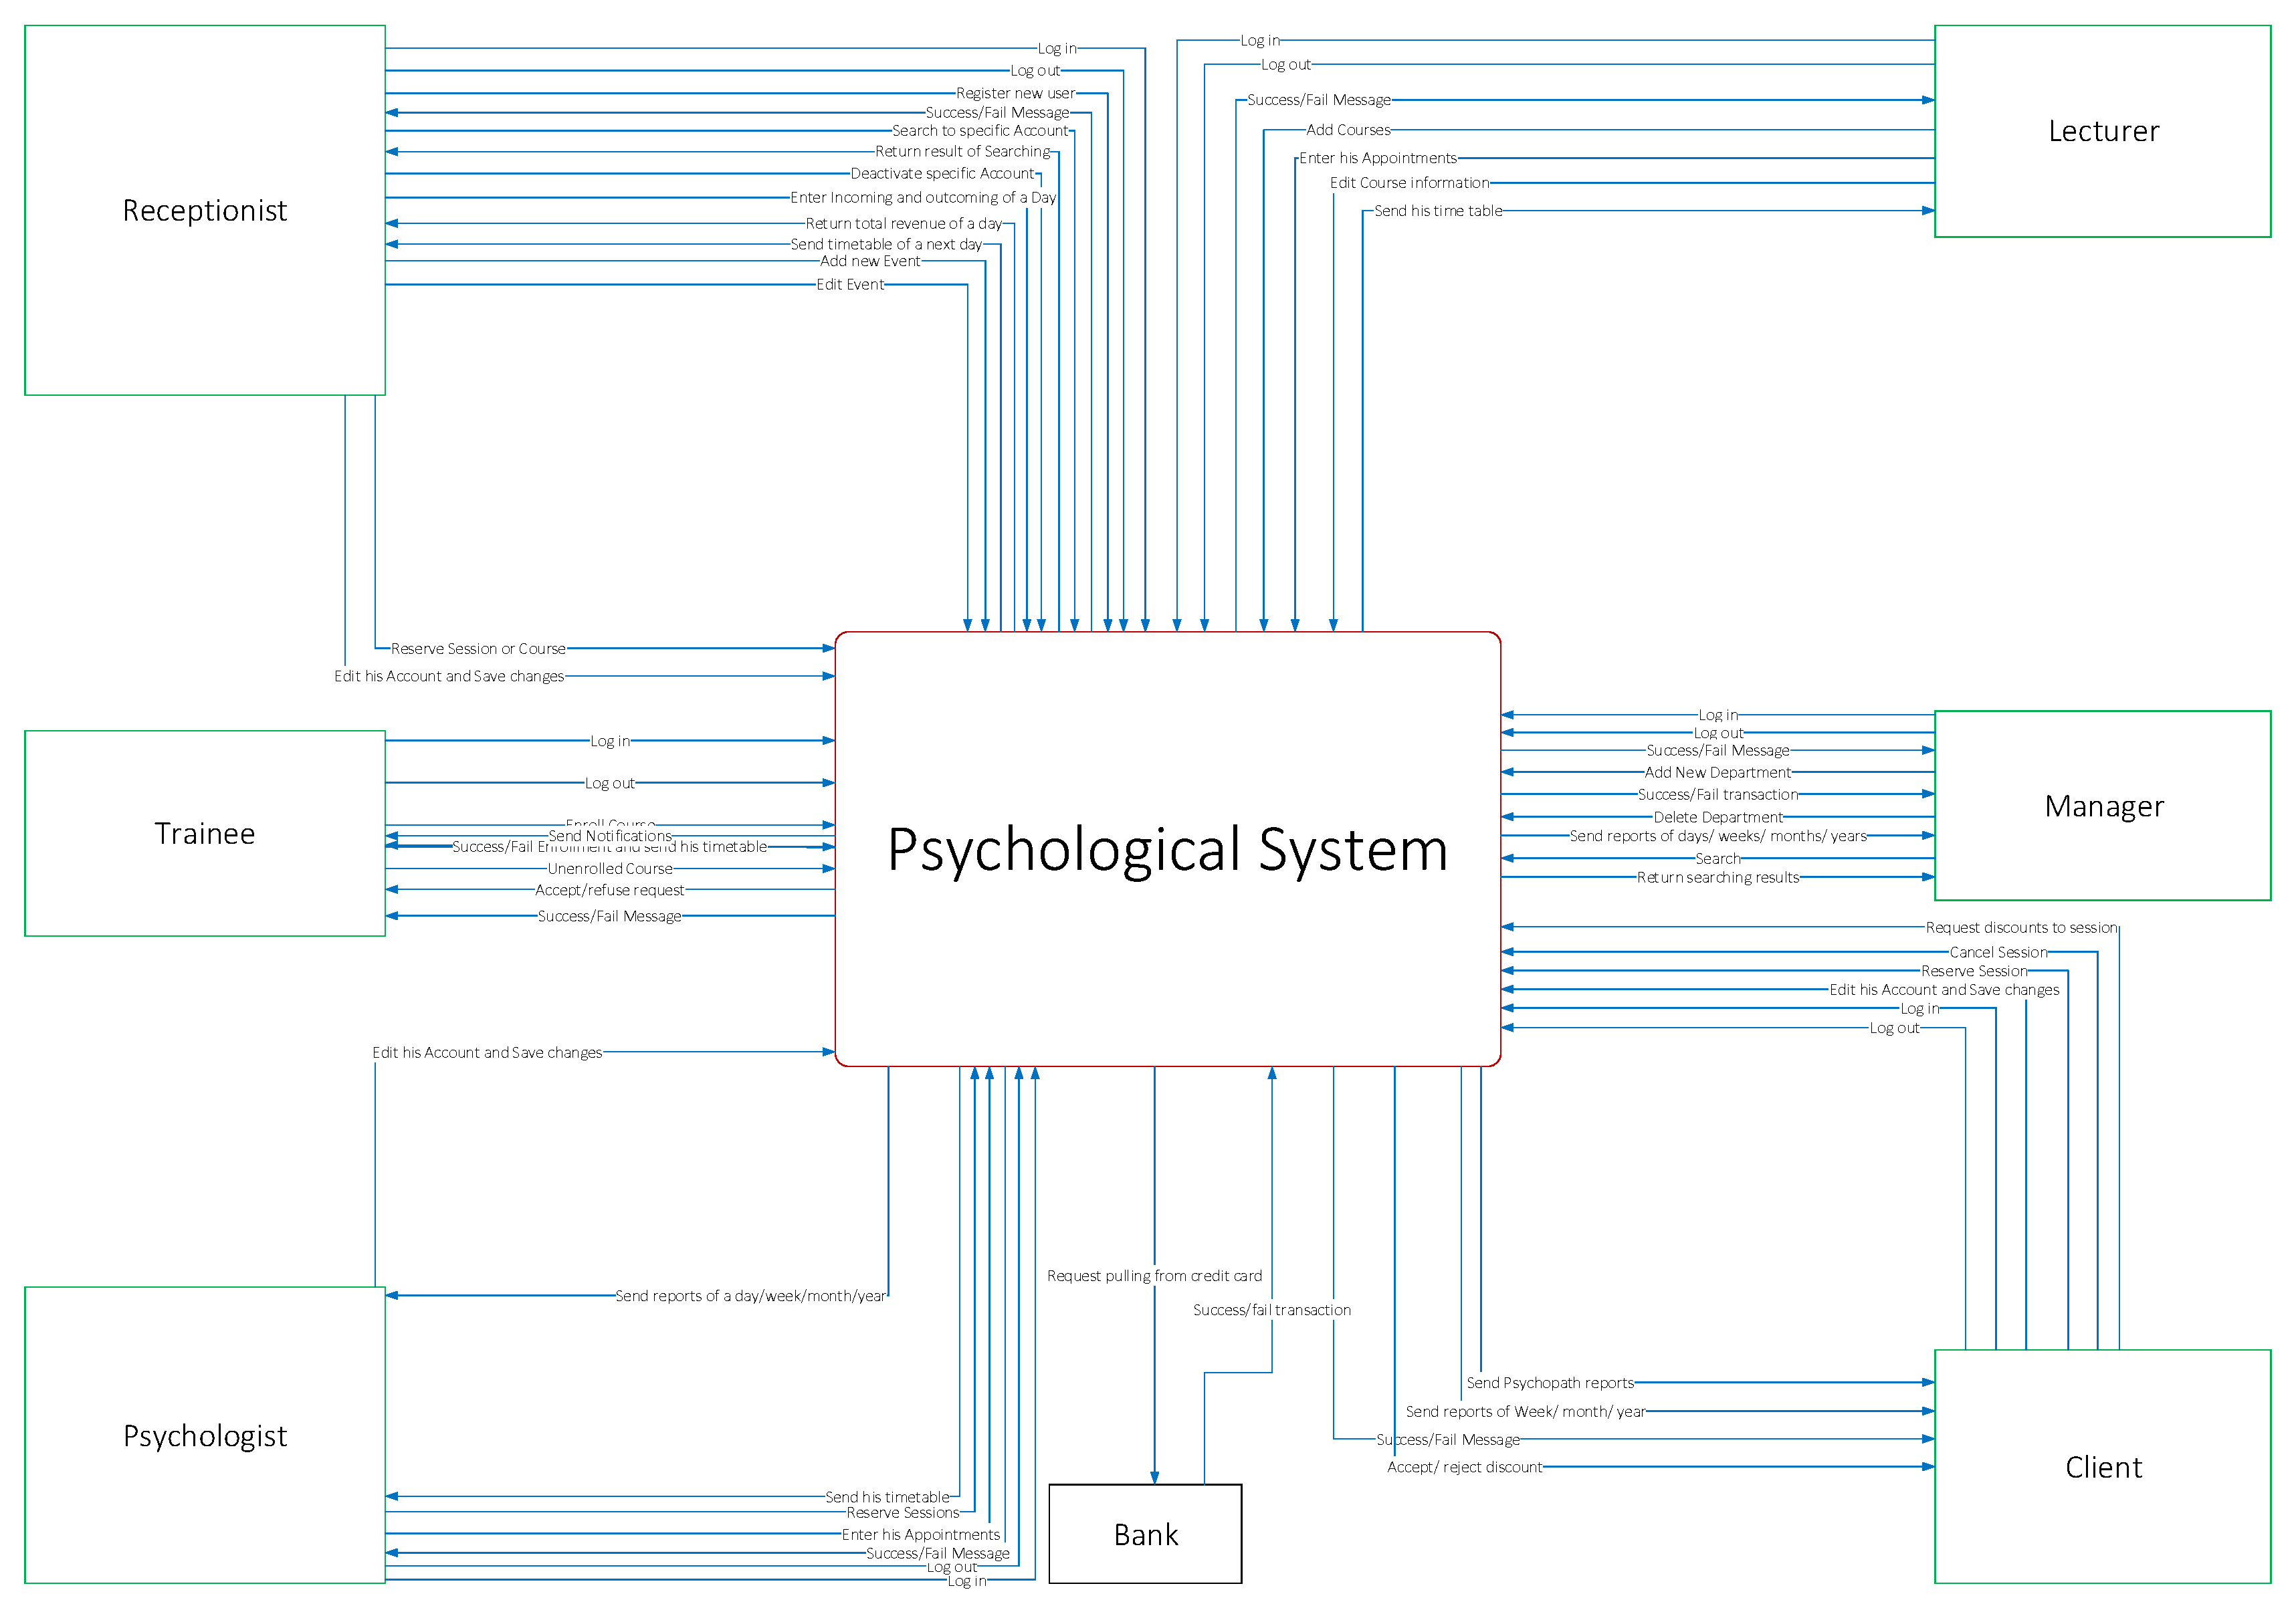
\includegraphics[width=\textwidth ,height=0.9\textheight ,scale=4]{Diagrams/Data-Flow_Context.pdf}
					
				\subsubsection{level one}
					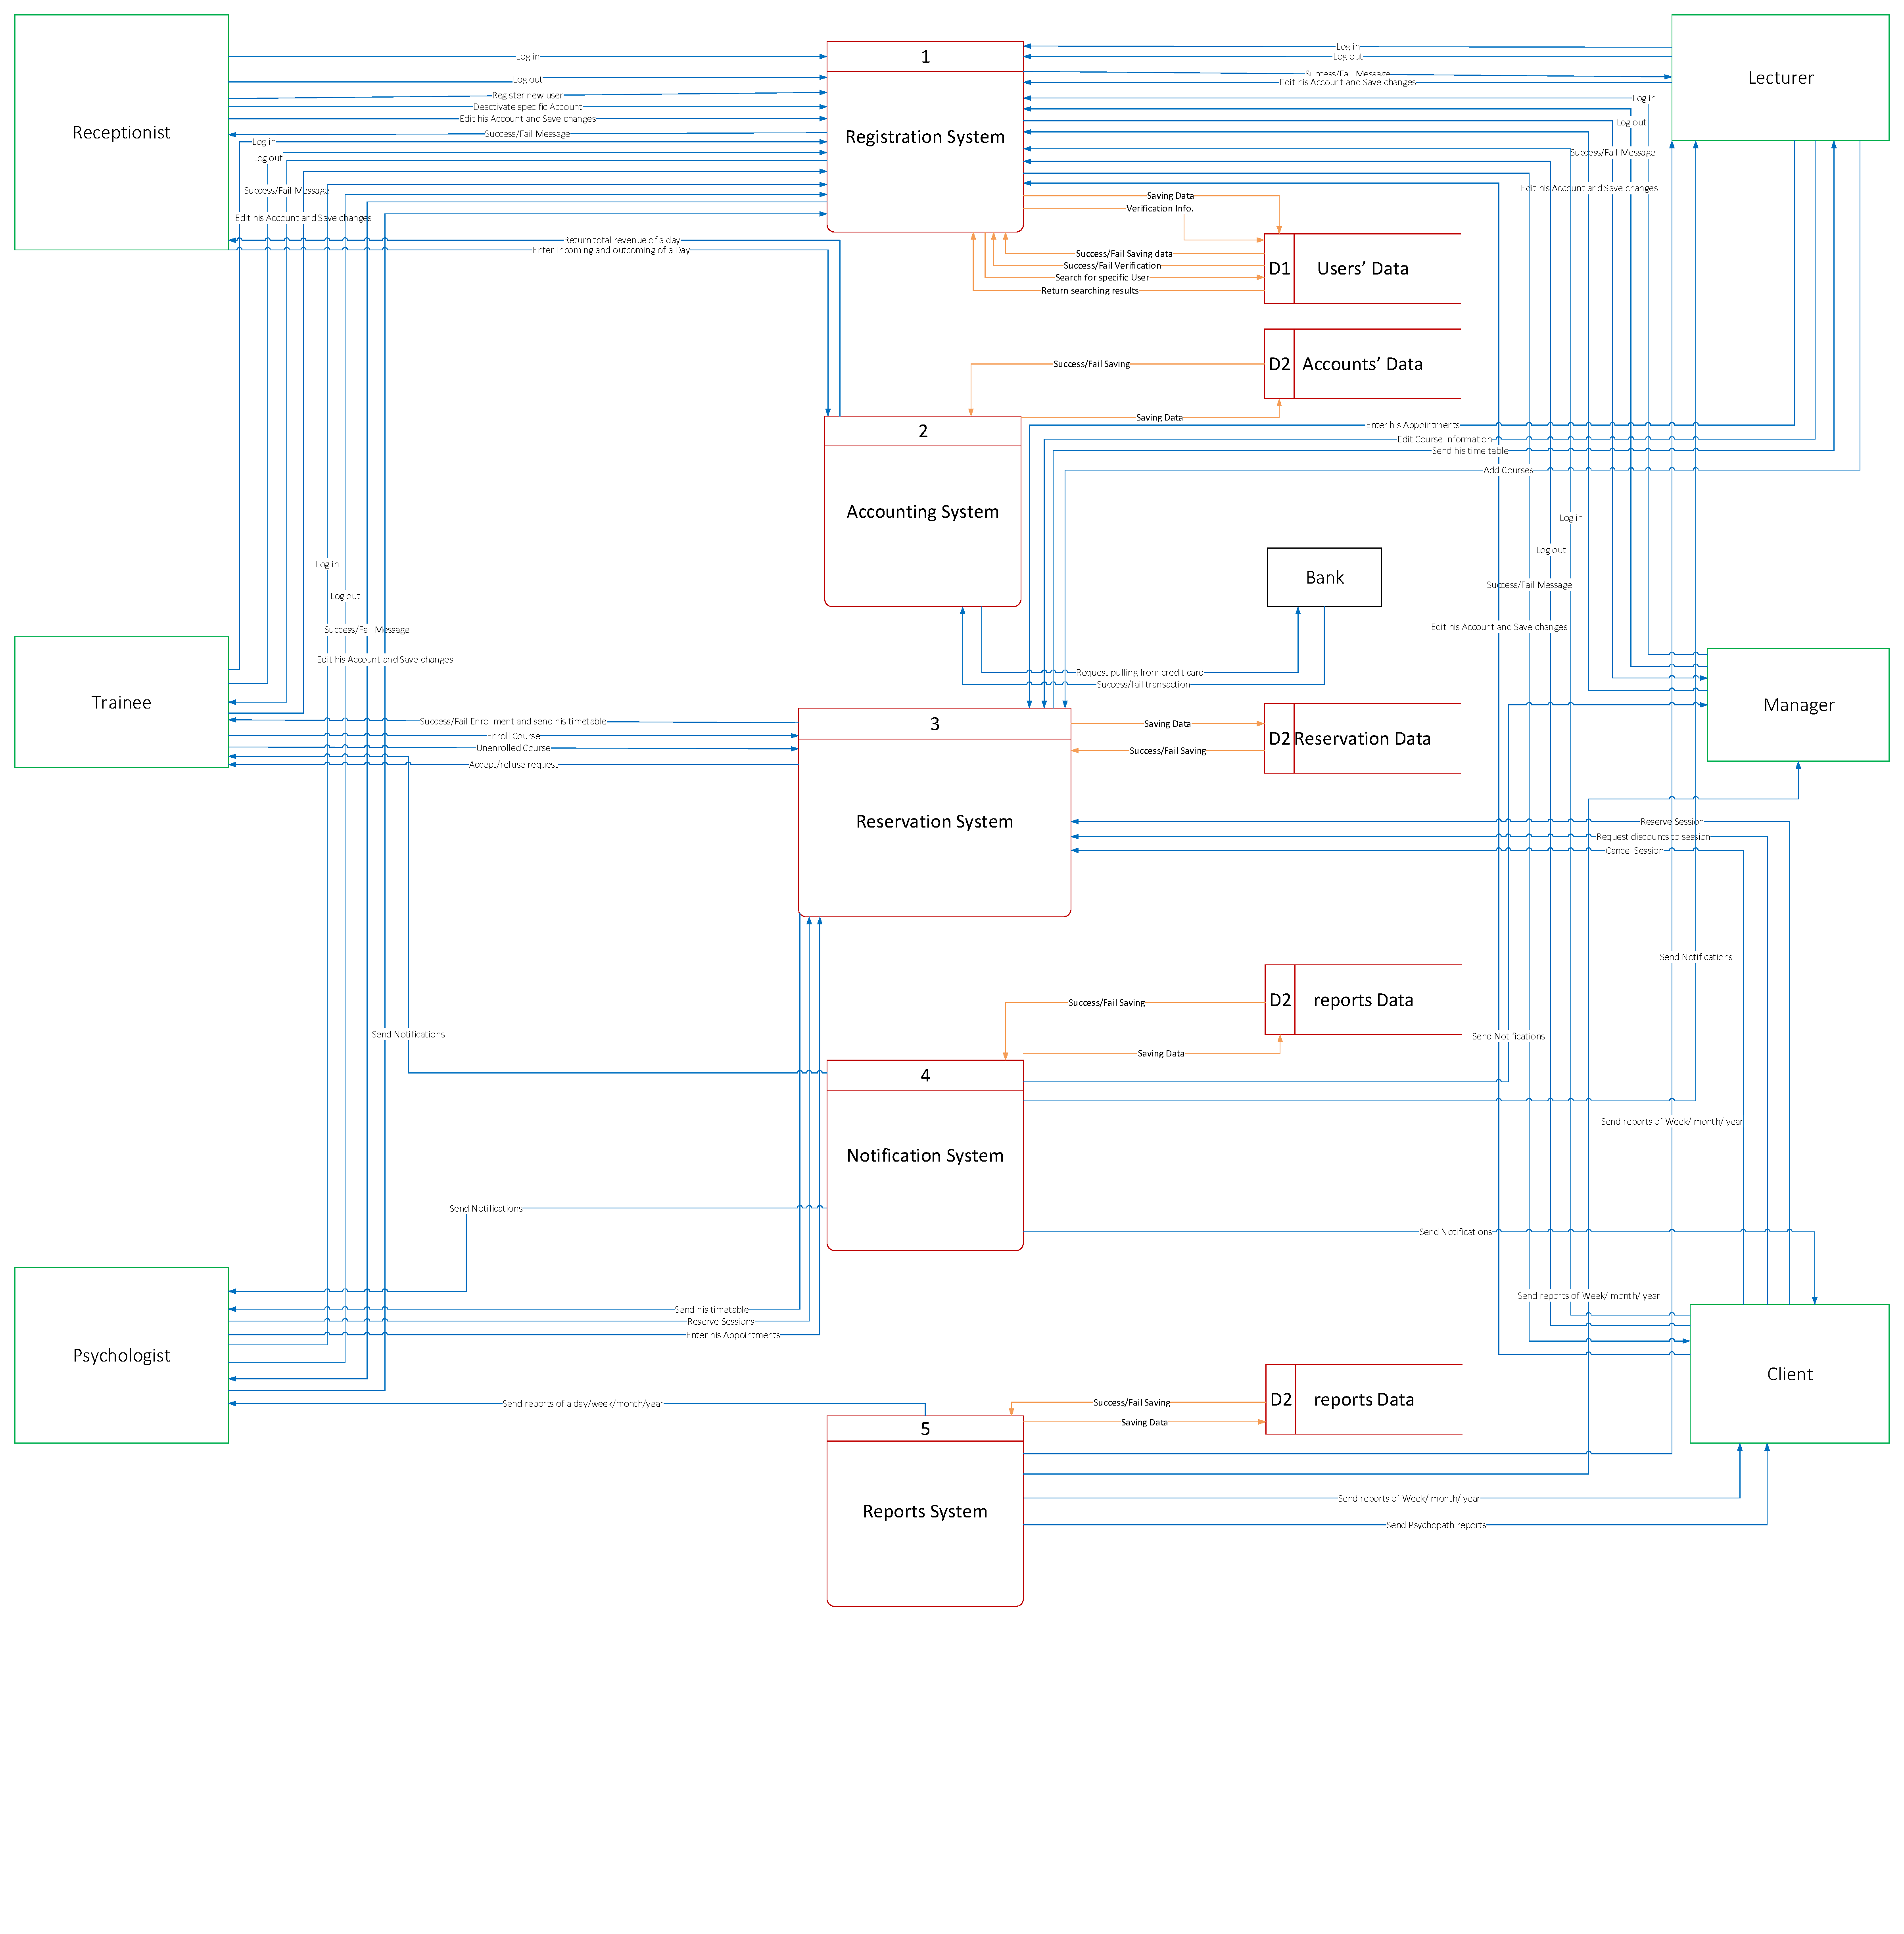
\includegraphics[width=\textwidth ,height=0.9\textheight ,scale=4]{Diagrams/Data-Flow_level0.pdf}
					
					
				\subsection{Use case diagram}
					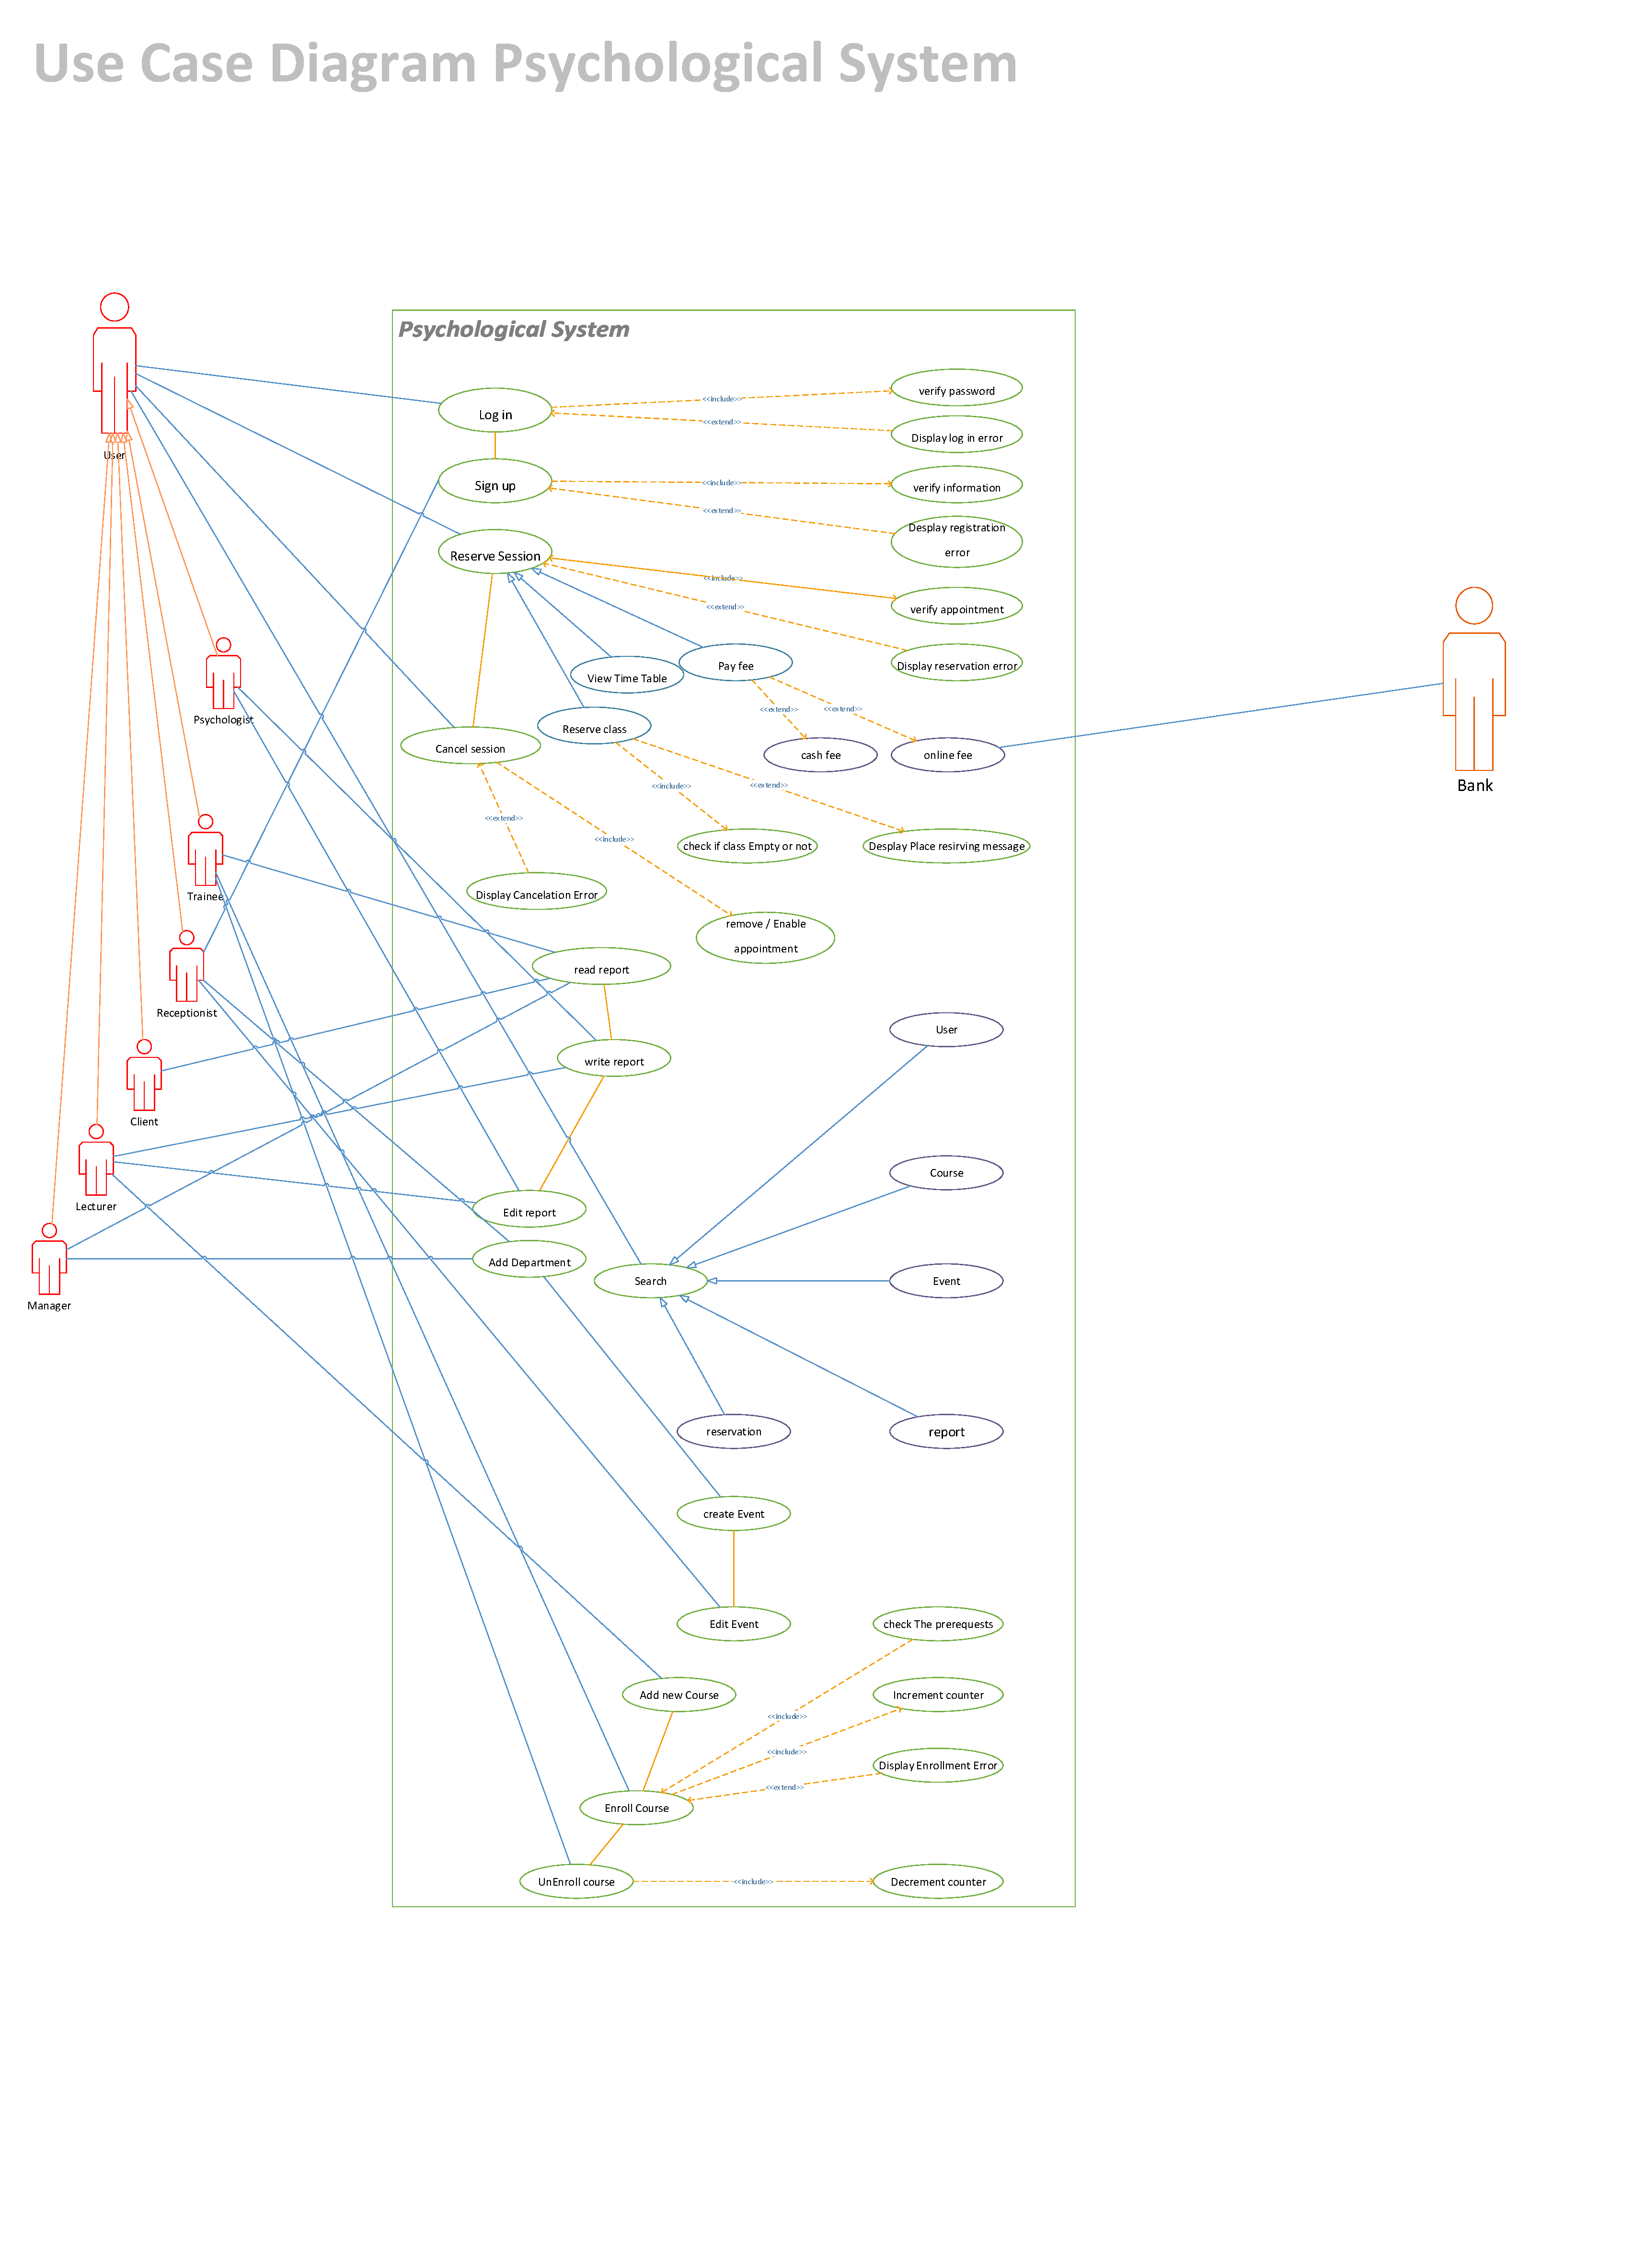
\includegraphics[width=\textwidth ,height=0.9\textheight ,scale=4]{Diagrams/use_case_psychological_system.pdf}
					
				\subsection{Class diagram}
					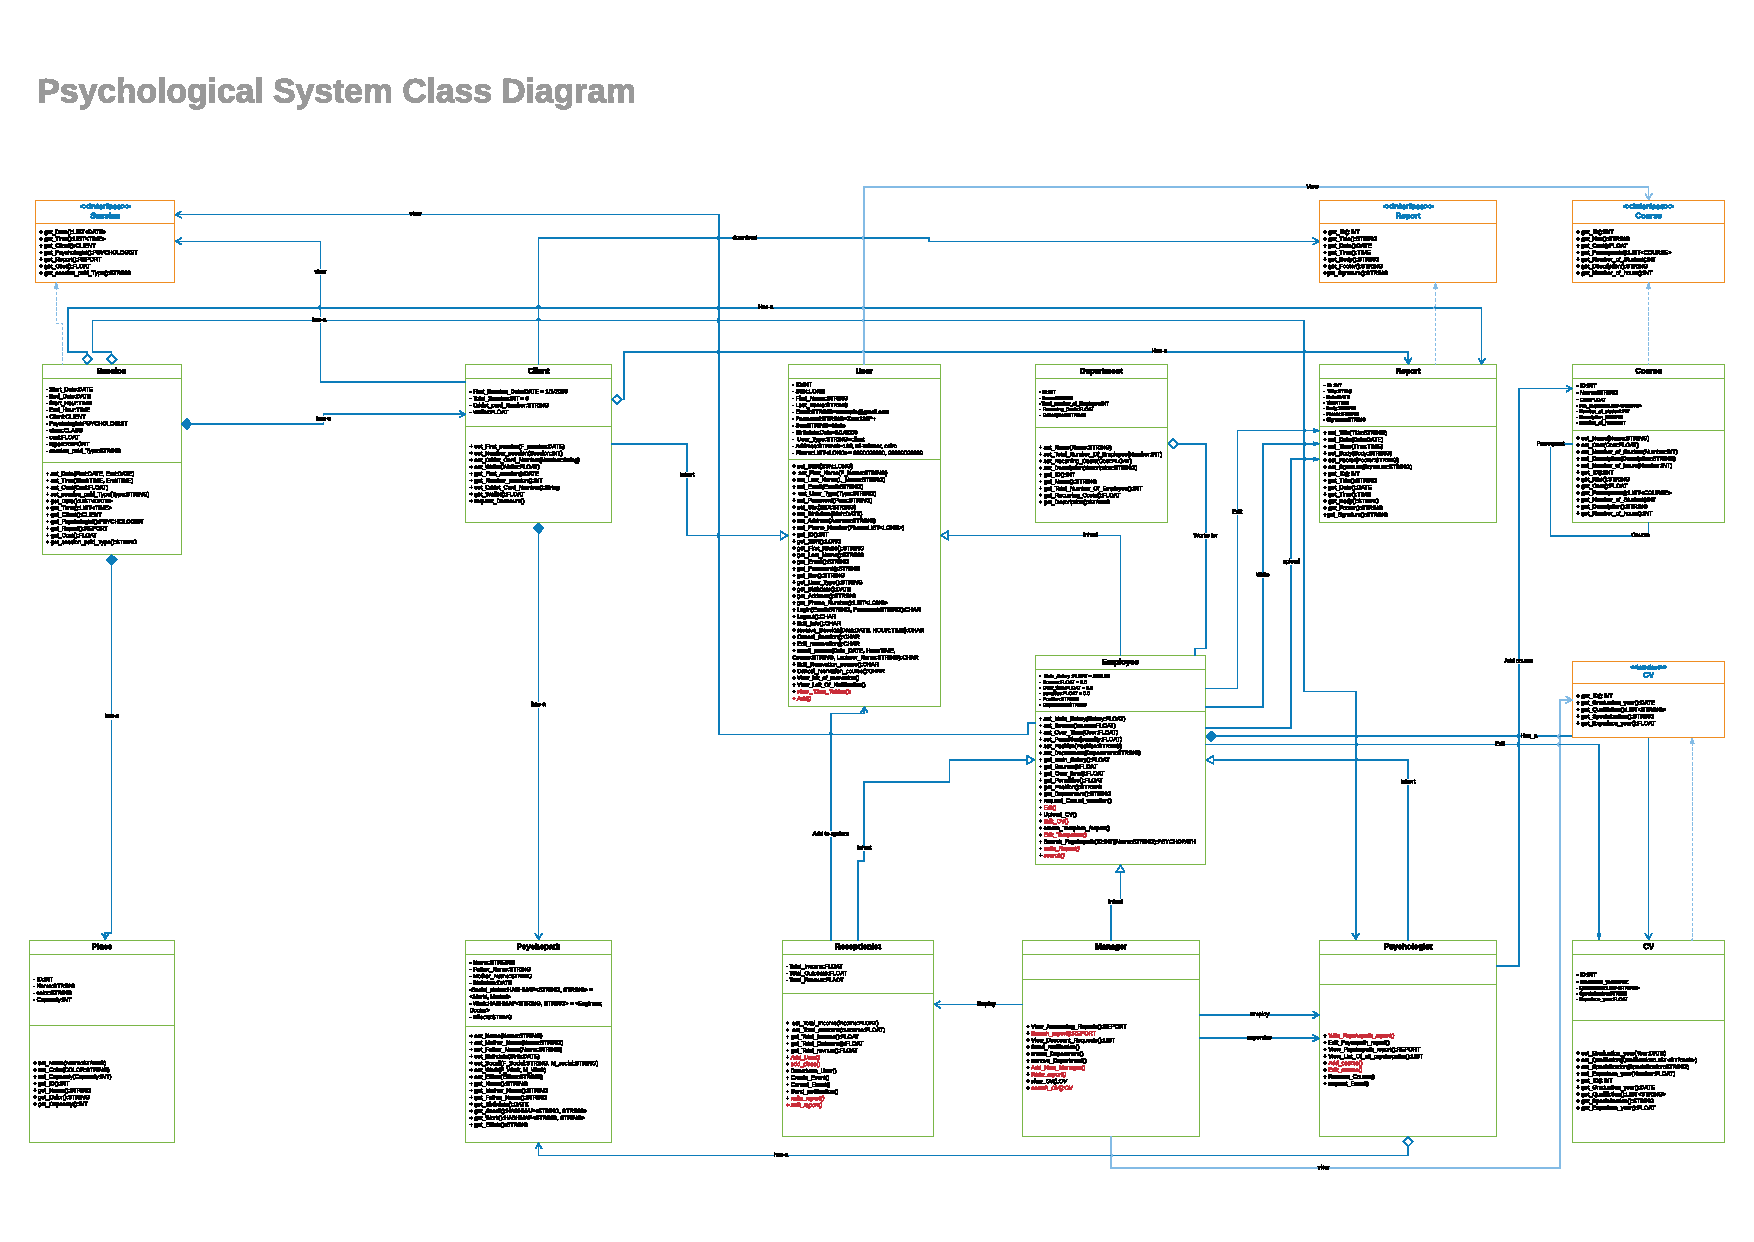
\includegraphics[width=\textwidth ,height=0.9\textheight ,scale=4]{Diagrams/Class_Diagram_for_Psychological_System.pdf}	
					
					\subsection{Activity Diagram}
					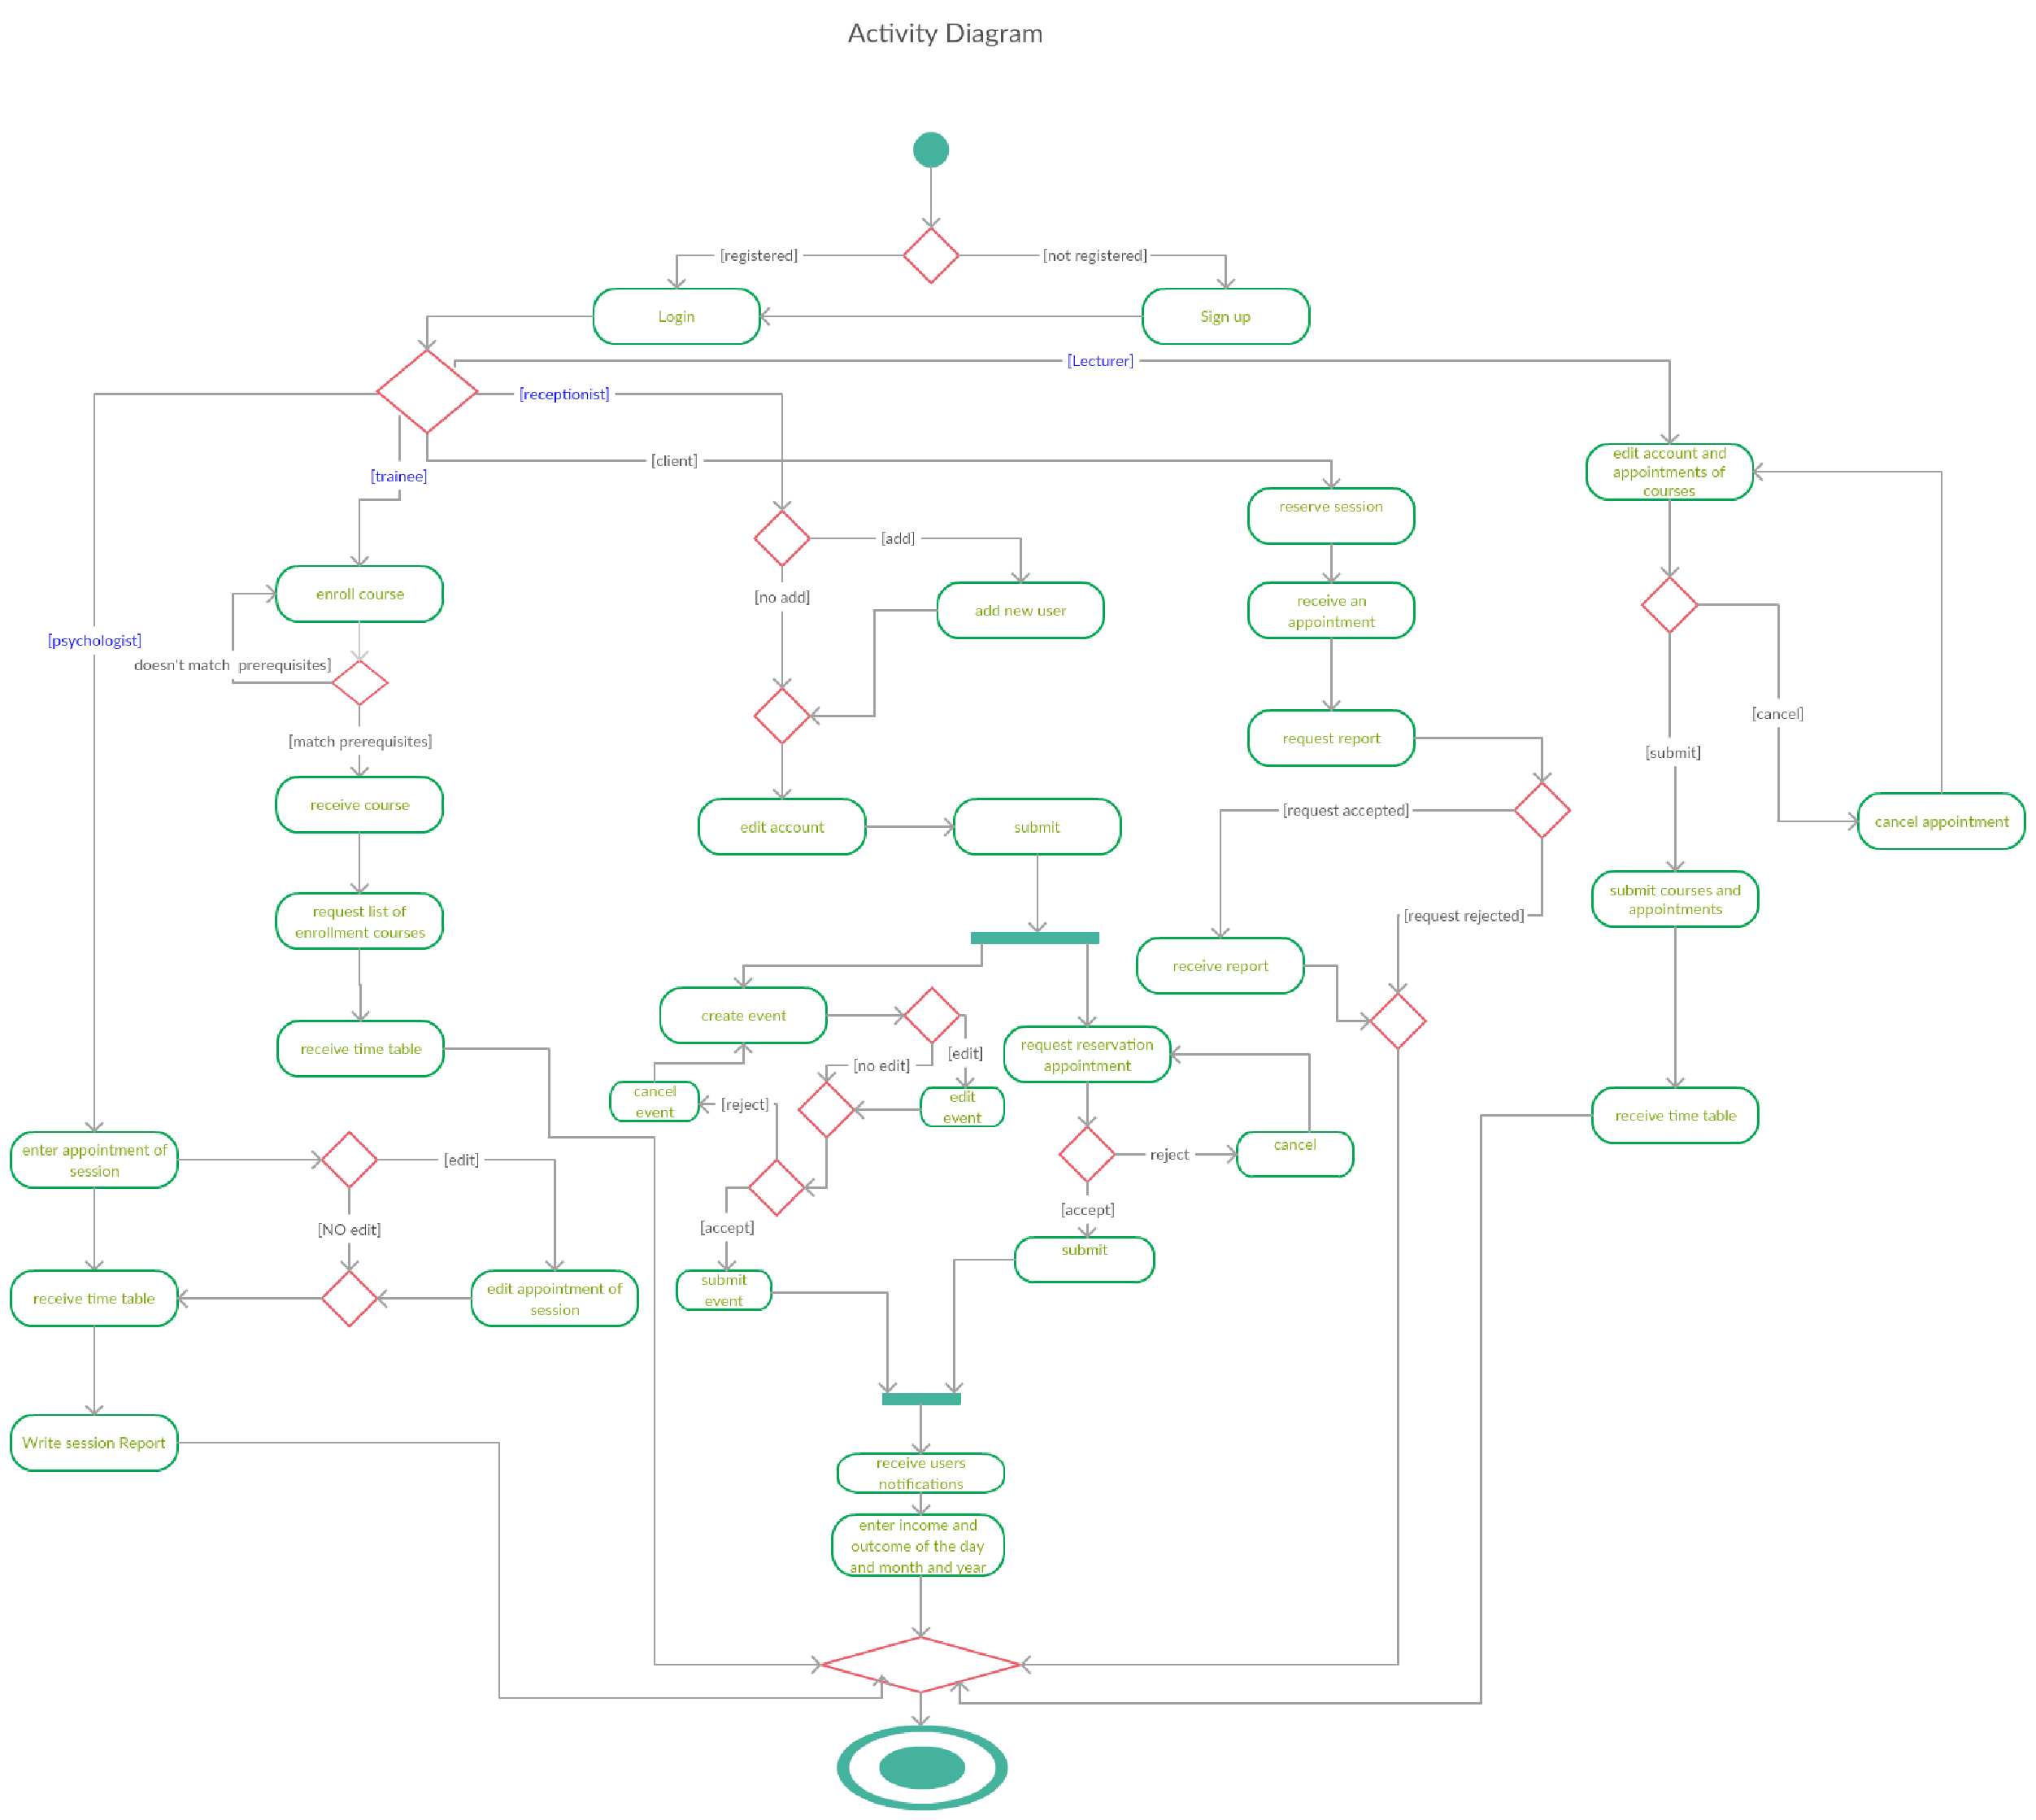
\includegraphics[width=\textwidth ,height=0.9\textheight ,scale=4]{Diagrams/Activity_Of_Psychological_System.pdf}	
					
%%%%%%%%%%%%%%%%%%%%%%%%%%%%%%%%%%%%%%%%%%%%%%%%%%%%%%%%%%%%%%%%%%%%%%%%%%%%%%%%%%%%%%%%%%%%%%%%%%%%%%%%%%%%%%%%%%%%%%%%%%%%%%%%%%%%%%%%%%%%%%%%%%%%%%%%%%%%%%%%%%%%%%%%%%%%%%%%%%%%%%%%%%%%%%%%%%%%%%%%%%%%%%%%%%%%%%
		\section{ASSUMPTION DEPENDENCIES}
			\paragraph{Let us assume that this is an Inelegant psychological System and it is used in the following application:}
				\subsection{For Management system}
					\begin{itemize}
							\item
								\textbf{\textsc{\color{red}Manager}}
									\begin{itemize}
						\item
							\textbf{\textsc{\color{blue}connect with Employees and supervise them.}}
						\item
							\textbf{\textsc{\color{blue}connect with clients and monitoring motions of organization.}}
						\item
							\textbf{\textsc{\color{blue}veiw all reports that specified to Calculations and salaries of Employees and Exports resources ...etc.}}
						
					\end{itemize}
							\item
								\textbf{\textsc{\color{red}Receptionist stuff}}
									\begin{itemize}
										\item
											\textbf{\textsc{\color{blue}create an account for new user.}}
										\item
											\textbf{\textsc{\color{blue}make reservation of appointment or course to specific client.}}
										\item
											\textbf{\textsc{\color{blue}recourd sessions per day and help you in the calculations.}}
						
									\end{itemize}
					\end{itemize}
				
				\subsection{For clinic system}
				\begin{itemize}
					\item
							\textbf{\textsc{\color{red}client:}}
					\begin{itemize}
						\item
							\textbf{\textsc{\color{blue}A request for booking session with specific specialist.}}
						\item
							\textbf{\textsc{\color{blue}choosing from available appointments for his specialist.}}
						\item
							\textbf{\textsc{\color{blue}View his specific reports to his case and results, plans, and solving to issues that specified to his case.}}
						\item
							\textbf{\textsc{\color{blue}update or cancel his resrvation, and update his profile.}}
					\end{itemize}
					
					\item
							\textbf{\textsc{\color{red}Specialist:}}
							\begin{itemize}
							\item
								\textbf{\textsc{\color{blue}Enter his appointments to the system.}}
							\item
								\textbf{\textsc{\color{blue}update and delete any appointment belongs to him, and update his profile.}}
							\item
								\textbf{\textsc{\color{blue}upload the reports that specified to his cases and upload his plan of treatment.}}
							\item
								\textbf{\textsc{\color{blue}connect with cases and receptionist.}}
					\end{itemize}
				\end{itemize}
				
				\subsection{For academic system}
				
					\begin{itemize}
					\item
							\textbf{\textsc{\color{red}Trainee:}}
					\begin{itemize}
						\item
							\textbf{\textsc{\color{blue}A request for booking course.}}
						\item
							\textbf{\textsc{\color{blue}choosing from available appointments for the course that he Enrolled it.}}
						\item
							\textbf{\textsc{\color{blue}system should rtrive to him his schedule.}}
						\item
							\textbf{\textsc{\color{blue}update or cancel his resrvation, and update his profile.}}
					\end{itemize}
					
					\item
							\textbf{\textsc{\color{red}Trainer:}}
							\begin{itemize}
							\item
								\textbf{\textsc{\color{blue}Enter his appointments for the courses to the system.}}
							\item
								\textbf{\textsc{\color{blue}update and delete any appointment belongs to him, and update his profile.}}
							\item
								\textbf{\textsc{\color{blue}upload the reports of result that specified to his trianees and upload scoring to them.}}
							\item
								\textbf{\textsc{\color{blue}generate some tests and help trainer in correcting this tests.}}
					\end{itemize}
				\end{itemize}
		
%%%%%%%%%%%%%%%%%%%%%%%%%%%%%%%%%%%%%%%%%%%%%%%%%%%%%%%%%%%%%%%%%%%%%%%%%%%%%%%%%%%%%%%%%%%%%%%%%%%%%%%%%%%%%%%%%%%%%%%%%%%%%%%%%%%%%%%%%%%%%%%%%%%%%%%%%%%%%%%%%%%%%%%%%%%%%%%%%%%%%%%%%%%%%%%%%%%%%%%%%%%%%%%%%%%%%%
\end{document}